\documentclass[11pt]{article}
\usepackage{amsmath,amssymb,booktabs,tabularx}
\usepackage{algorithm,algpseudocode}
\usepackage{hyperref}
\usepackage[preprint]{acl}
\usepackage{times,latexsym}
\usepackage[T1]{fontenc}
\usepackage[utf8]{inputenc}
\usepackage{microtype,inconsolata,graphicx,tikz,pgfplots}
\usetikzlibrary{arrows.meta,positioning,fit,calc}
\pgfplotsset{compat=1.18}
\newcommand{\code}[1]{\texttt{#1}}
\newcommand{\project}{SSA-HPM}
\title{Software-Semantic-Aware Hardware Performance Monitoring}
\author{Liu Qinruo}
\hypersetup{pdftitle={Software-Semantic-Aware Hardware Performance Monitoring},pdfauthor={Liu Qinruo},pdfsubject={Calling-context attribution and Linux lifecycle on a single-hart RISC-V Rocket prototype},pdfkeywords={RISC-V, Rocket, hardware performance monitoring, calling context, Linux, memory classification}}
\begin{document}
\maketitle
\begin{abstract}
Hardware counters summarize execution but provide limited information about the software path responsible for an event. SSA-HPM combines hardware-assisted hierarchical calling-context tracking with context-associated counters, Linux session management and offline reconstruction on a RISC-V Rocket core. Supported calls and returns invoke private microcode that maintains a context stack, dictionary and records. Inclusive cycle, time and retired-instruction intervals are supplemented by one native DTLB or D-cache event profile. A bounded retirement observer classifies integer memory accesses using per-session virtual-address histories. Trusted Linux hooks preserve open frames across scheduling, separate exec images and export frozen sessions in checked chunks; a controlled launch policy enables audited ordinary ELF targets automatically. Public-baseline reconstruction, 34 directed RTL cases, six Spike reference cases and actual Rocket/Verilator Linux runs establish the supported behavior. Independent performance experiments provide 150 bare-metal and 150 Linux work samples, with all results matching closed-form arithmetic. In the call-heavy bare workload, basic monitoring increases the median from 1,088 to 46,328 cycles, or 42.58 times the disabled runtime; long memory loops amortize the cost to approximately 0.80\% and 0.40\% increases. The implementation and evidence form a reproducible single-hart research baseline with explicit lifecycle, capacity and measurement semantics.
\end{abstract}
\section{Motivation and Objectives}
Performance counters expose properties of execution such as cycles, retired instructions and requests to the memory hierarchy. Their interpretation depends on software context. A function reached through two parent paths can have different data, working sets and reuse behavior. A flat function count merges these paths, while a global counter also includes activity from other tasks and privileged handlers. Hierarchical context records make those distinctions explicit.

\project{} investigates a hardware-assisted connection between normal RISC-V calls and those measurements. The target is an inspectable Rocket implementation integrated with the Chipyard simulation environment~\citep{rocket,chipyard}. Application calls trigger helper execution in the core, rather than requiring an inserted monitoring call at each function. A trusted Linux component controls selection and lifetime, and an offline tool reconstructs a context tree from exported records. This arrangement makes architectural behavior, software ownership and measurement boundaries testable together.

The project has four concrete objectives. First, retain parent/callee identity through nested calls, repeated paths, returns and architectural traps. Second, associate the basic counters and selected native memory-hierarchy events with those contexts while excluding sampled scheduling pauses. Third, implement an executable definition for scalar, stream and irregular memory accesses at retirement. Fourth, provide a complete Linux-to-host result path, including automatic launch of selected ordinary executables and explicit handling of exec, exit and incomplete sessions.

The completed prototype addresses these objectives on one hart. Validation combines directed RTL programs, independently reconstructed retirement observations, actual Linux process execution and host protocol mutations. Performance evaluation uses independently sampled target counters around reproducible bodies. The result is both an implementation and an evidence set: source baselines, ordered patches, configuration hashes, native return codes, shutdown markers and semantic checkers identify what was executed.

The public project entry is \url{https://github.com/Kimberley-Inti/ssa_hpm}. The accepted implementation is tagged \code{v0.2.0}; documentation and this report are a presentation follow-up that preserves its implementation and evidence. Functional navigation groups calling contexts, process accounting, event attribution, export, classification and launch policy, while original development identifiers remain in historical records.

\subsection{Design Basis}
The original project brief describes a procedure-call stack, a parent-sensitive context dictionary and performance records, followed by dataflow objectives for memory patterns and Cache/TLB events~\citep{designbrief}. It proposes a 36\,MiB context region associated with a loader-managed application stack and a small helper-code store named SCCodeTable. Several OS and offline-analysis details are left open.

The implementation makes those open points explicit. Kernel-owned physical pools replace application stack mappings; generated private ROMs implement the helper-code concept; session identity separates tasks and images; and bounded checked streams carry records to host files. Rule 1 defines the address-pattern decision, and the two native profiles define exactly which hardware handshakes increment the fourth counter. These choices form the operating contract described in the following sections.

The accompanying editable report follows the supplied ACL preprint layout and bibliography mechanism~\citep{acltemplate}.

\section{System Architecture and Implementation}
\label{sec:architecture}
\subsection{Hardware and Software Boundaries}
Figure~\ref{fig:architecture} shows the end-to-end path. The Rocket pipeline recognizes supported calls and returns and executes the corresponding private helpers. The helpers maintain context structures in a selected pool and read counter snapshots. Native event signals feed the ordinary HPM machinery. A separate retirement observer updates bounded per-session memory-pattern state. The Linux layer selects a pool, preserves and restores open-frame accounting, and freezes results before export. Host tools validate the stream and build software context trees.

\begin{figure*}[t]
\centering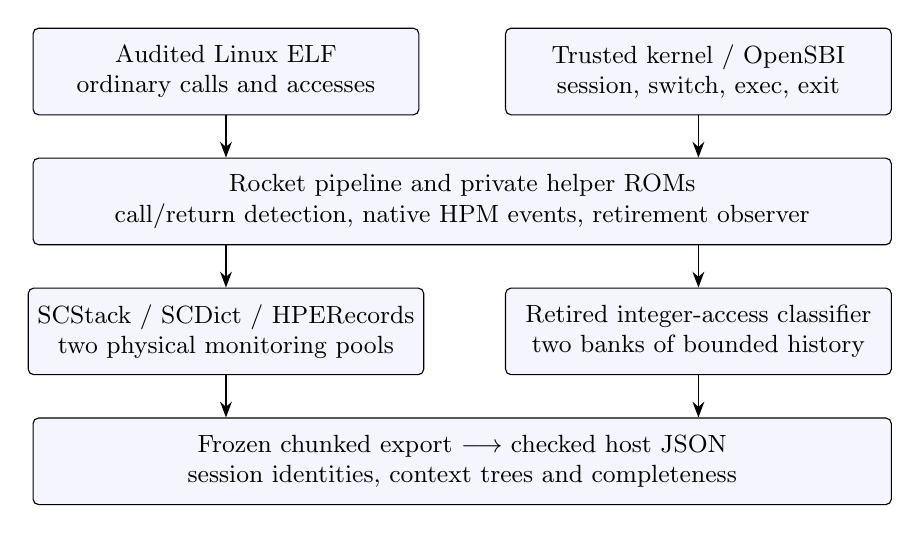
\begin{tikzpicture}[font=\small,box/.style={draw,rounded corners=2pt,align=center,minimum height=11mm,fill=blue!4},arr/.style={-{Stealth[length=2mm]},semithick}]
\node[box,minimum width=49mm] (app) at (0,0) {Audited Linux ELF\\ordinary calls and accesses};
\node[box,minimum width=49mm] (os) at (6,0) {Trusted kernel / OpenSBI\\session, switch, exec, exit};
\node[box,minimum width=109mm] (core) at (3,-1.65) {Rocket pipeline and private helper ROMs\\call/return detection, native HPM events, retirement observer};
\node[box,minimum width=49mm] (mem) at (0,-3.3) {SCStack / SCDict / HPERecords\\two physical monitoring pools};
\node[box,minimum width=49mm] (class) at (6,-3.3) {Retired integer-access classifier\\two banks of bounded history};
\node[box,minimum width=109mm] (host) at (3,-4.95) {Frozen chunked export $\longrightarrow$ checked host JSON\\session identities, context trees and completeness};
\draw[arr] (app.south)--(core.north -| app);
\draw[arr] (os.south)--(core.north -| os);
\draw[arr] (core.south -| mem)--(mem.north);
\draw[arr] (core.south -| class)--(class.north);
\draw[arr] (mem.south)--(host.north -| mem);
\draw[arr] (class.south)--(host.north -| class);
\end{tikzpicture}

\caption{Implemented data and control paths. Calling-context helpers update physical-pool structures; the classifier maintains its own bounded banks. Linux controls ownership and lifetime, and offline reconstruction consumes frozen versioned results.}
\label{fig:architecture}
\end{figure*}

The source delivery is an independent repository of patches and project files. It reconstructs public Chipyard, Rocket, Linux and OpenSBI baselines rather than depending on a development VM's private Git objects. The configured hardware is \code{SSAHPMEventRocketConfig}, with one Rocket hart and a 40-bit event counter. Generated L1 instruction and data caches are each 16\,KiB, with 64 sets, four ways and 64-byte lines. A CLINT supplies the timebase. The Linux and firmware versions are 5.7-rc 3 and 0.8 respectively~\citep{linux,opensbi}.

\subsection{Call Detection and Helper Execution}
The supported calling convention uses \code{x1} or \code{x5} as link registers and matching return forms. Architectural instruction decoding, including decompressed instructions, identifies the relevant \code{JAL}/\code{JALR} behavior. A normal jump remains a jump. Calls and returns under the monitoring policy invoke private helper sequences, with the original architectural operation completed coherently around them.

The helpers use a private integer-register bank. This protects application-visible registers while scratch values hold dictionary addresses, record IDs and counter deltas. ROM execution is serialized with architectural retirement and memory operations. Directed register-transparency tests exercise ordinary argument/saved registers, alternate-link calls and jumps; workload results provide an additional functional cross-check.

The original SCCodeTable proposal stores a few helper routines for hashing, lookup, creation and accounting. The prototype realizes this as generated constant microcode ROMs from one canonical assembly source. The basic and event variants contain 104 and 118 words respectively, or 888 bytes combined. A generation/check step detects divergence between the assembly and Scala ROM representation. Writable runtime SRAM loading is a potential extension of this storage mechanism.

\subsection{Context Structures}
SCStack contains open activations. A64-byte frame carries the record ID and entry snapshots, with the event snapshot present for ABI2. Its supported full-tree depth is 256. A return reads the current frame, adds counter deltas to the associated record and restores the parent. Repeated activation of an already known context therefore adds to one record rather than allocating a new path each time.

SCDict maps $(p,a)$, where $p$ is the parent record ID and $a$ is the callee's full virtual target address. The implemented hash uses shifted address bits XORed with the parent, selecting one of 262,144 buckets. A1\,MiB bucket table contains 32-bit links to record chains. Chain comparison checks the full key, retaining separate paths when hashes collide. Context IDs are allocated monotonically; ID0 is reserved. Capacity checks protect record-space boundaries.

HPERecords have 128-byte slots. The first two 64-bit fields are callee and parent, followed by cycle, instret and time counts at offsets 16,24 and 32. ABI2 uses record offset 40 for the fourth event. Other fields support chain links and reserved space. There are 262,144 slots per pool, giving 262,143 usable IDs. Two fixed 36\,MiB pools reserve 72\,MiB in total. Releasing a session makes its slot available for reuse; the physical carve-outs remain reserved.

\subsection{Identity and Trap State}
A context path is local to a monitoring session. Same-address functions in two processes or two exec images are separated by pool/session ownership, even when their numerical record IDs coincide. Raw virtual addresses identify code within that image; ELF-linked fixture checks provide names where available. The general result format retains addresses and image identity independently of optional symbolization.

Architectural trap state belongs to the hart. Handler calls are suppressed from the application tree, and notification resumes at the appropriate architectural return. Privilege and overflow checks keep private helper state coherent. Application context filtering and counter source filtering are distinct: a handler can be absent from the tree while its work still contributes to a surrounding inclusive interval. Linux scheduling adds the explicit pause exclusion described next.

\section{Calling Contexts and Event Accounting}
\label{sec:accounting}
\subsection{Inclusive Counter Intervals}
RISC-V exposes basic cycle, time and instruction-retirement counters and programmable HPM facilities with privilege-controlled access~\citep{riscvpriv,riscvunpriv}. The implemented basic snapshots are 64 bits. For counter $C$ of width $w$, an activation with entry $b$ and exit $e$ contributes
\begin{equation}
 d_C=(C(e)-C(b))\bmod 2^w.
\label{eq:interval}
\end{equation}
The corresponding record accumulates these deltas across repeated activations. A parent remains open during its child calls, so its interval includes descendants and helper/handler work occurring between its own sample points. Counter ordering and helper boundaries determine which setup/return work lies inside an interval.

The basic time field uses CLINT time. Architectural Linux \code{rdtime} reads are supplied by OpenSBI on this Rocket configuration, while the private measurement path can access the platform timer. Counter-access permissions control who may read a CSR; they do not themselves remove privileged events from the global source.

\subsection{Native Event Profiles}
ABI2 adds one 40-bit HPM snapshot and result. A firmware image fixes its meaning. The DTLB profile uses selector \code{0x1002}. Rocket's \code{io.dmem.perf.tlbMiss} is connected in DCache to \code{io.ptw.req.fire()}, so this profile counts accepted page-table-walker request handshakes. Walk completion and eventual instruction retirement are downstream observations.

The Cache profile uses selector \code{0x202}. DCache assigns \code{io.cpu.perf.acquire} from \code{edge.done(tl\_out\_a)}: the final accepted beat completes an outbound TileLink-A request message. This measures traffic through the D-cache A port, including qualifying PTW and uncached requests. Response/refill completion is a different point in the transaction. The actual signal and EventSet path, rather than a shorthand event label, define the profile~\citep{rocketimpl}.

Both profiles attribute increments by sampled execution interval. An in-flight request can complete its A message after a call or return boundary; the context open when that increment is sampled receives it. This provides a reproducible interval metric using the existing global counter. Precise request-origin attribution would additionally require carrying a context tag with the request. The exported profile, width and selector make the implemented rule explicit.

Arithmetic uses the hardware width. For a 40-bit counter moving from $2^{40}-2$ to 3, the modular delta is 5. Directed RTL fixtures exercise wrap and verify that unrelated architectural registers remain unchanged. Firmware and kernel profile definitions agree on selector and width before a Linux session is enabled.

\subsection{Excluding a Scheduling Pause}
A task can be switched out with several frames open. Let $S_j$ and $R_j$ be the outgoing and incoming samples for a pause, and let
\begin{equation}
 q_{C,j}=(C(R_j)-C(S_j))\bmod 2^w.
\end{equation}
Software adds $q_{C,j}$ to every open frame's entry snapshot. Its eventual completed interval becomes
\begin{equation}
 d_C=\left(C(e)-C(b)-\sum_j q_{C,j}\right)\bmod 2^w.
\label{eq:rebase}
\end{equation}
The stack, dictionary and current context remain in the task's pool; global counter registers keep running. Unmonitored tasks run with selection 0. Samples are ordered counter reads, so each counter uses its own measured pair. Work before $S_j$ and after $R_j$, including sampling/restore instructions outside those points, remains in the task's interval.

\begin{figure*}[t]
\centering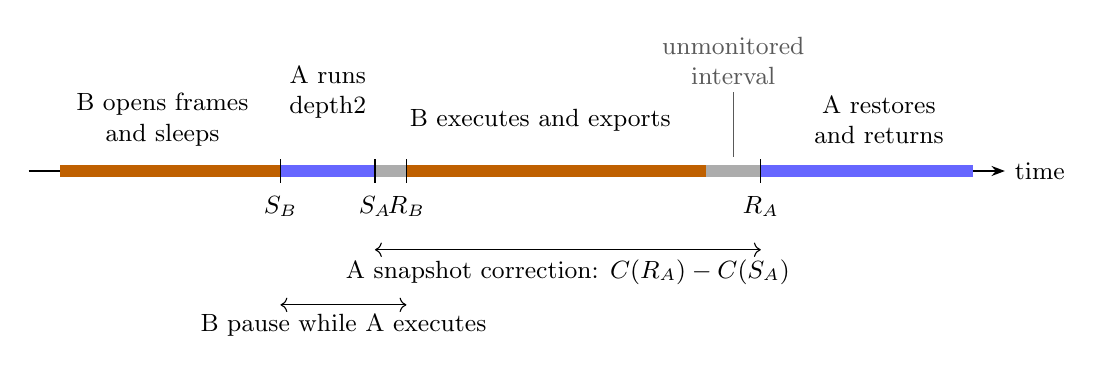
\begin{tikzpicture}[font=\small,x=1cm,y=1cm,arr/.style={-{Stealth[length=1.7mm]},semithick}]
\draw[arr] (0,0)--(12.4,0) node[right]{time};
\draw[line width=4pt,orange!75!black] (.4,0)--(3.2,0);
\draw[line width=4pt,blue!60] (3.2,0)--(4.4,0);
\draw[line width=4pt,gray!65] (4.4,0)--(4.8,0);
\draw[line width=4pt,orange!75!black] (4.8,0)--(8.6,0);
\draw[line width=4pt,gray!65] (8.6,0)--(9.3,0);
\draw[line width=4pt,blue!60] (9.3,0)--(12,0);
\node[align=center] at (1.7,.65) {B opens frames\\and sleeps};
\node[align=center] at (3.8,1.0) {A runs\\depth2};
\node at (6.5,.65) {B executes and exports};
\node[align=center] at (10.8,.65) {A restores\\and returns};
\foreach \x/\s in {3.2/S_B,4.4/S_A,4.8/R_B,9.3/R_A}{\draw (\x,-.15)--(\x,.15);\node[below] at (\x,-.2) {$\s$};}
\draw[<->] (4.4,-1.0)--node[below]{A snapshot correction: $C(R_A)-C(S_A)$}(9.3,-1.0);
\draw[<->] (3.2,-1.7)--node[below]{B pause while A executes}(4.8,-1.7);
\node[align=center,gray!70!black] at (8.95,1.4) {unmonitored\\interval};
\draw[gray!70!black] (8.95,1.0)--(8.95,.18);
\end{tikzpicture}

\caption{Schematic ordering for the real timer-wakeup test, with $S_B<S_A<R_B<R_A$. A has two open frames at its timer-driven switch-out. Gray segments denote kernel/unmonitored handoff work. Distances are illustrative rather than proportional to measured cycles.}
\label{fig:scheduling}
\end{figure*}

Cache pollution illustrates the difference between exclusion and isolation of microarchitectural state. B's increments during A's sampled pause are subtracted from A. After A resumes, its own accesses can encounter cache lines displaced by B; their new events belong to A's active interval. The protocol provides record/history ownership and interval accounting while retaining a shared cache/TLB hierarchy.

\subsection{Observable Context Relationships}
The canonical fixture calls \code{parent\_a} and \code{parent\_b}, both of which call \code{common}. It also creates two intentionally colliding functions. The six records consist of two parent records, two parent-specific common records and two collision records. On repeated paths the common counts are 14,452 and 7,226 retired instructions. Their relationship, distinct parent IDs, restored parent depth and collision-chain links are checked against the raw RTL output, rather than inferred from a success label alone.

\section{Linux Integration and Lifecycle}
\label{sec:linux}
\subsection{Session Ownership and Interfaces}
The experimental kernel interface is enabled for the single-hart MMU configuration. A task descriptor owns its pool, session/image identity, excluded-interval state, open frames and switch diagnostics. Local interrupt exclusion protects selection and state transitions. Hart counters and trap notification state remain hardware resources. The user interface accepts operations on the current task, without a user-supplied PID or physical pool address.

The principal operations are START, STOP, EXPORT and ARM\_EXEC. START initializes an available pool and selects its ABI/profile state. STOP requires zero open/spilled frames, samples the cutoff and disables selection. EXPORT accepts a stopped session and emits its frozen records. Diagnostic operations expose selected state for tests. The trusted automatic-exec operation arms policy for a selected future image. The implementation preserves ABI1's three counters and ABI2's event field.

Scheduler hooks implement Equation~\ref{eq:rebase}. Switch-out records task state, peer IDs, frame depth/RID and trap causes, samples the counters and clears selection. Switch-in samples again, corrects every open snapshot and reselects that task's pool and classification epoch. An absent descriptor leaves monitoring disabled. Frozen or stopped descriptors are not resumed by scheduling.

\subsection{Successful and Failed Exec}
An image replacement has a commit point beyond which execution will not return to the old image~\citep{linuxexec}. Monitoring retirement is tied to this boundary rather than to the initial exec request. The old session is frozen, its closed records are retained, and its remaining open activations are exported with abandoned status. The slot stays owned through terminal output. Descriptor release and slot reuse follow that export.

The new image receives a clean dictionary/stack/session and a reset classification epoch when monitoring is enabled. Manual operation leaves enablement to the new image; the armed launch policy enables it when the replacement ELF is ready. Session ID plus the kernel's image generation distinguishes results under the same PID and prevents old snapshots from entering the new session.

A repeatable pre-commit failure uses a missing executable and returns ENOENT. The old program then continues within its original open frame and ultimately returns normally. Its descriptor, context tree and history remain intact; there is no premature export or pool release. The validation records this returning failure separately from successful image replacement.

\subsection{Stop, Exit and Pool Reuse}
Normal exit and default signal termination freeze active sessions, export them and release the descriptor/slot. Explicit STOP can retain a frozen result until EXPORT, with repeated export rejected. An already exported result is not emitted again at exit. Open frames at an exit or exec commitment identify unfinished activations; closed records retain their completed counts without fabricating a normal return for the open portion.

During export the task stays STOPPED and the selected pool is disabled. Interrupts and scheduling can resume another task on its own pool while chunks are printed. The exporting pool remains busy until its terminal record and release step, preventing a new session from resetting the data mid-transfer. With both slots busy, a selected third task receives an observable enable failure and continues according to the documented fail-open test policy.

\subsection{Controlled Automatic Launch}
A trusted launcher configures an exec policy while it has CAP\_SYS\_ADMIN and sets \code{no\_new\_privs}. It then drops uid/gid for the audited target. The target's source and ELF contain ordinary code without monitoring lifecycle calls. A successful ELF-ready hook establishes the session before user execution. Tests retain target hashes and disassembly checks, including static executables, a musl PT\_INTERP image and a shared library~\citep{musl}.

Fork clears the child's descriptor and launch policy, so a child obtains a separate session only through a new eligible policy/START operation. The fixtures reject unsupported thread/setid paths and verify that unselected executables remain unmonitored. Automatic-exec inheritance is explicit; failed pre-commit replacement preserves the old image/session. The tested dynamic loader and application share a session. One audited musl continuation leaves a loader frame abandoned, which remains visible in the exported lifecycle state.

\subsection{Real Preemption and Direct Proof}
The two-task fixture uses a timer wakeup: B sleeps while A executes with two open frames, then a higher-priority B becomes runnable. Saved interrupt cause 5, runnable A state, increased involuntary-switch count and peer identities establish the switch. Ordered raw samples show $S_B<S_A<R_B<R_A$ as in Figure~\ref{fig:scheduling}. A continues its original call after resuming and both tasks return with independent records.

A separate two-record companion reads actual original/final frame snapshots for all four counters. It is needed because the inherited diagnostic prints SSA\_ACCOUNT only when exactly two context records exist, whereas the full performance task also calls a third memory-body function. The companion uses matching kernel/firmware trees, measurement configuration and the same RTL executable, while retaining the real streamed/irregular memory work. The default full benchmark's loadable bytes were independently recompiled and confirmed unchanged after adding this conditional fixture.

For A, the excluded amounts are 4,463,467 cycles,3,429,517 instructions,44,635 time ticks and 12,115 Cache events. B excludes 132,475 cycles,117,572 instructions,1,325 ticks and 147 events. These values equal final-minus-original frame snapshots and independently summed S/R deltas modulo width. The emitted raw column is a reconstructed uncorrected estimate, so the direct proof rests on frame memory and independent samples. Host mutations reject missing/duplicate counter rows and incorrect sample/offset values.

\section{Retired Memory-Access Classification}
\label{sec:classification}
\subsection{Observation and State}
The design brief lists scalar, streaming and random accesses but leaves their executable decision rule open. Rule 1 defines a bounded local address-pattern classifier. It observes valid architectural integer load/store instructions of widths 1,2,4 or 8 bytes at Rocket writeback. The effective address and instruction PC are virtual. Validity excludes replay, exceptions and cancellation; private helper code and kernel instructions under the Linux user-only policy are excluded. FP, vector, atomic/LRSC and page-table-walker operations have separate semantics outside this observer.

Each history key contains session epoch, HPERecord ID, PC, load/store kind and access width. Two hardware banks correspond to the two owned pools. Each bank has 16 fully associative history entries with FIFO replacement, a 256-depth record-ID stack mirror and 63 usable counter rows. Record 0 represents access outside a framed activation and is reported separately. Five 64-bit counters per row record input, warmup, scalar, stream and irregular totals.

The key separates interleaved instructions, access widths and calling paths. A repeated call to the same context can continue its history. Replacement discards only the evicted local pattern state; its next observation starts warmup again and the eviction count is exported. Record-row overflow produces an explicit dropped/coverage diagnostic, rather than assigning an out-of-range row to its parent.

\subsection{Rule 1 Decision}
For one key, the first two observations are warmup. Subsequent accesses compare the new virtual-address delta with the previous delta, using 64-bit address arithmetic. Equal zero deltas produce scalar-repeat. Equal nonzero signed deltas produce stream-fixed-stride when magnitude is at most 4,096 bytes and divisible by the access width. All remaining observations are irregular/unrecognized. Every accepted input receives exactly one of these categories.

\begin{table}[t]
\centering\small
\begin{tabular}{ll}\toprule
Virtual-address sequence & Rule 1 outputs\\\midrule
$0,0,0,0$ & W,W,S,S\\
$0,8,16,24$ & W,W,T,T\\
$32,24,16,8$ & W,W,T,T\\
$0,32,8,80,0$ & W,W,I,I,I\\
$0,0,0,8,16,24$ & W,W,S,I,T,T\\\bottomrule
\end{tabular}
\caption{Examples for one 8-byte-access key. W is warmup, S scalar-repeat, T stream and I irregular/unrecognized. Separate PCs have separate histories.}
\label{tab:patterns}
\end{table}

Table~\ref{tab:patterns} illustrates first access and a mode transition. Alternating two independent PCs preserves each pattern, while alternating unrelated addresses at a single key can remain irregular. The category describes a recognized local address relationship. Statistical randomness or a dominant whole-program pattern would require a different classifier and validation criterion.

\subsection{Context and Lifecycle Semantics}
Classification counters are exclusive to the current record. An inclusive view can be reconstructed by summing a record's descendants, whereas HPM records already include child intervals. Both representations are exported with their aggregation semantics. This distinction avoids treating a parent's own memory operations as equivalent to all work beneath it.

A disabled selection observes no task accesses. Task switches restore the appropriate bank/history and record stack; no HPM-style pause subtraction is needed for these source-filtered per-context counts. A new exec session resets its epoch after the previous export/release, and a returning pre-commit failure keeps the old history. The Linux test checks open-frame switching, same-address functions in independent tasks, exec separation and complete sidecar export.

An independent Python implementation supplies the address-rule oracle. RTL-directed patterns cover fixed addresses, positive/negative strides, irregular sequences, mode changes, interleaved streams, parent-sensitive contexts, repetition and replacement/capacity. A read-only pre-clock writeback observer reconstructs actual accepted memory observations independently of the classifier's result. Its capture contains 82 candidates,72 accepted accesses,7 replay candidates and 1 exception. Reference comparison and semantic negative controls check category totals and context ownership against these real sequences.

\section{Result Export and Offline Reconstruction}
\label{sec:export}
\subsection{Frozen, Bounded Transfer}
The export stream carries the semantic records needed to reconstruct calling contexts. Unused pool slots and dictionary buckets remain internal implementation state. A frozen descriptor retains ownership while the kernel maps and copies at most 16 records, or 2,048 bytes, at a time. Each chunk is emitted and unmapped before continuing; scheduling can proceed between chunks without enabling the exporting session again.

A version 1 session header identifies session, PID, image generation, pool, ABI, allocated record total, capacity, chunk size, active counters, event profile and accounting policy. Counter descriptors name each quantity, width and selector. Chunk headers carry sequence, first ID and count. Each record contains ID, parent, callee, counters and open-activation count. Per-chunk and whole-session word checksums detect missing or changed transfer content, and the terminal header reports emitted/expected counts and integrity state.

The checksum folds 64-bit words using $h\leftarrow(h\mathbin{\mathrm{xor}}x)\times 1099511628211$ modulo $2^{64}$ from an agreed initial value. It is a corruption check within a trusted capture path. Semantic oracles additionally verify expected relationships even when a negative test repairs the checksum after changing ownership. Internal chunk reads validate the current task/descriptor, session, frozen/busy state and record bounds, with a maximum count of 16.

\subsection{Independent Completeness Dimensions}
Transport completion, call completion and classification coverage are represented independently. A complete record stream can include an abandoned frame from exec or exit. Closed records stay settled; unfinished activations retain their identities and entry snapshots rather than acquiring fabricated return counts. A separate coverage state identifies dropped classification rows, overflow, history replacement and unframed observations.

Classification sidecars have their own rule version, observation scope, aggregation mode, bounded-state metadata, rows and terminal checksum. The current base header declares whether the sidecar is required and its expected row count. This repairs a gap where losing a whole optional sidecar could evade transport-only checks or cause a semantic lookup error. Historical captures without the declaration remain explicitly identified as legacy data.

The pool stays owned until terminal output and release. Explicit stop/export is one-time; exec and exit follow their distinct lifecycle paths before freeing the descriptor. Source filtering and selector state keep hardware updates away from frozen data. These ownership rules make a stable bounded transfer possible without copying an entire 36\,MiB pool or running a huge UART dump.

\subsection{Host Reconstruction and Tests}
Python tools parse the stream into session-local records and resolve parent links into calling-context trees. They check metadata, widths, sequence/order, duplicate or missing IDs, declared totals, checksums, dangling parents and session boundaries. The output preserves counter definitions and completeness states. Fixture-specific symbol information can name addresses; raw address identity remains available for general offline analysis.

Actual Rocket/Linux export includes a 41-record session in three chunks, two-record and zero-record sessions, explicit stop, abandoned frames and exec reuse. The production validation also exports 64 records in four chunks and a 105-record dynamic session in seven chunks. In the 64-record case, base records are all transferred while classifier capacity stops at 63 rows and reports the dropped access. Host protocol tests cover missing chunks, duplicates, truncation, bad checksums/ranges and absent declared sidecars. Maximum-capacity arithmetic and full serial enumeration are recorded as different coverage levels.

\section{Experimental Setup and Correctness Validation}
\label{sec:evaluation}
\subsection{Pinned Construction and Provenance}
Validation runs in an Ubuntu 22.04 VM using RISC-V GCC 15.1.0, Verilator 4.226, Spike 1.1.1-dev, Java 17 and Python 3.12.12. Fixed public source revisions are fetched before project patches are applied. Existing matching Chipyard dependency and musl 1.2.5 caches are reused after verification; target fixtures, the final RTL model, kernels and firmware are actually built. The full reproduction entry is scripts/final.py reproduce; scripts/final.py check-evidence replays saved evidence without target execution. REPRODUCE.md lists prerequisites and exact commands. The report data is extracted from committed evidence~\citep{ssahpm}.

\begin{table*}[t]
\centering\small
\begin{tabular}{lll}\toprule
Component & Public reconstruction baseline & Accepted development source\\\midrule
Chipyard &\scriptsize\texttt{2d03d10837fc1a7569d10ae2c91c8132c7fee77d}&\scriptsize\texttt{d756a546e27d40100752a0ff7c73b796c77d4fde}\\
Rocket Chip &\scriptsize\texttt{44b0b8249279d25bd75ea693b725d9ff1b96e2ab}&\scriptsize\texttt{bb5b1c26a8dae5d5afee716a1636b55a1bfe1ed2}\\
Linux &\scriptsize\texttt{5f5fd87b36e21ed59b759b69eebfa1c74955cb37}&\scriptsize\texttt{3e7c06efefeda043f100ab635b1729ce7a11afd8}\\
OpenSBI &\scriptsize\texttt{a98258d0b537a295f517bbc8d813007336731fa9}&\scriptsize\texttt{43f02ffb329d9c86b2ff2138dc450b2060778ffe}\\\bottomrule
\end{tabular}
\caption{Source identity. Reconstruction applies three Chipyard and fourteen Rocket patches in order, then installs standalone project files and selected Linux/firmware patches. Trees/hashes establish equivalence even when reconstructed committer metadata changes commit IDs.}
\label{tab:sources}
\end{table*}

A new workspace compiles Scala, generates RTL and builds the event-configured Verilator model. A separate progress harness links against its unchanged model archive and reads PC/CSR state; it does not modify RTL state. The final public-suite check verifies 111 source/document files and generated ROM consistency. Source/report presentation changes preserve the release implementation and raw evidence, with a historical reference map for renamed navigation.

Production, full-performance and direct-companion Linux payloads are built from matching kernel and OpenSBI source trees. The two measurement configurations match except their initramfs input path. A default-payload recompilation confirms that adding the conditional companion leaves the full benchmark's loadable bytes identical. An independent bare payload build likewise matches loadable bytes and non-FILE symbols; a temporary assembler-object name explains its differing non-loadable ELF metadata.

Every run stores its command, model/image hashes, native exit code, raw console output and checker result. Linux acceptance additionally requires normal powerdown and complete lifecycle/stream markers. Host replays, resealed mutations, reused dependency caches and earlier superseded trials have explicit labels. This avoids counting one saved capture as several hardware executions.

\subsection{Directed Hardware and Reference Matrix}
The final directed matrix contains 40 distinct cases: six Spike references and 34 Rocket RTL tests. Spike covers applicable instruction/ABI/reference behavior and has no SSA extension. The RTL cases exercise the actual implementation: nested calls, different parent paths, repeated-context reuse, return restoration, dictionary collisions, capacity guards, register transparency, trap/IRQ behavior, both event profiles, width/wrap handling and classification. Seven translation/permission probes are included in that count. Expected native-failure negative controls retain their actual status, including 42 where required.

An independent writeback oracle adds nine checks for real retired memory observations. It observes 82 candidates, accepts 72 and identifies seven replay candidates and one exception. Its reference comparison verifies that rejected/faulting operations do not become duplicate classified accesses. Category or context mutations supply further semantic negatives.

\subsection{Linux Matrix and Result Integrity}
The production Rocket/Linux boot naturally exits 0 and powers down normally. Its automatic-launch checker passes 51 checks and the manual compatibility checker passes 26. The same capture contains 17 sessions and 215 records, with every pool released. Independent postchecks add ten ELF-linked capacity checks, five automatic semantic negatives and three classification negatives. The static/dynamic ELF identities and their lack of SSA lifecycle calls are retained.

The production matrix covers selected and unselected programs, successful/failed exec, normal/default-signal exit, fork policy, unsupported thread/setid rejection, pool exhaustion, timer switching, history ownership, chunked export and visible partial states. A dynamic 105-record result includes an explicitly abandoned loader continuation. A 64-record result retains all HPM records while showing 63 classification rows, one dropped access and observable FIFO eviction.

Full Linux performance contributes 150 work samples and eight closed/released sessions containing 102 records. It observes actual timer/open-frame switching, but its three-record task has no inherited two-record-only snapshot diagnostic. The direct companion supplies the missing proof in another actual Linux run: two tasks, two sessions, four records and eight snapshot-account rows, with 20 checks passing. The composite checker keeps these coverage sources separate.

Review exposed and repaired two host issues in the new accounting oracle: variable initialization order and accepting eight rows without verifying the exact PID/counter identity set. The final negative suite has five host cases: one valid capture and four mutations for wrong delta, wrong offset, missing rows and duplicated counter coverage. All behave as expected after repair. Original failed postprocessing receipts remain available; successful native execution is reused. The complete evidence entry performs 12 host-only replay steps, including hash checks, result arithmetic and semantic oracles.

\section{Performance Evaluation}
\label{sec:performance}
\subsection{Protocol and Measurement Boundaries}
The experiment compares monitoring disabled, basic context accounting, DTLB, Cache, classification and matched Cache-plus-classification modes on the same extended model. Bare-metal runs use six modes. Linux uses off, basic, Cache, classification, manual Cache-plus-classification and automatic Cache-plus-classification. Automatic DTLB is outside this measured Linux matrix.

Five bodies represent different costs:128 arithmetic updates;128 leaf calls; depth 16 recursion; a 32\,KiB sequential read; and a 32\,KiB full-period irregular permutation. Data words are initialized as $17j+3$ and remain read-only during measured bodies. Each workload/mode has one unmeasured warmup and five measured repetitions, giving 150 work samples in each environment. There are 30 empty calibration samples in each experiment and six bare setup observations. Closed-form arithmetic independently verifies all 300 work results.

Ordered cycle/instret/time reads bracket the call and completed return, with console output outside the work interval. Empty samples are retained rather than blindly subtracted. Bare time uses direct CLINT MMIO; Linux \code{rdtime} takes the OpenSBI emulation path. The three reads are non-atomic: the cycle/instruction interval includes the first time-read emulation and excludes the second, while the time interval has slightly shifted endpoints. Those measurement costs remain consistent across modes.

Linux cost probes are optional at compile time and are disabled in the production regression image. They measure dictionary/metadata/selector initialization, freeze, bounded record copying, full export, switch hooks and exec windows. Pause/resume observations are deferred until frozen export, avoiding scheduler-path printing. Instrumented descriptors are 4,368 bytes versus 3,768 bytes by default; event diagnostics are 176 versus 128 bytes. These figures describe the instrumented build, with probe/cache/allocation effects retained.

\subsection{Bare-Metal Runtime and Instruction Cost}
\begin{table*}[t]\centering\small
\begin{tabular}{lrrrrrr}\toprule
Workload & Off & Base & DTLB & Cache & Class. & Cache+class.\\\midrule
Compute & 1,697 & 2,025 & 2,080 & 2,092 & 2,028 & 2,087\\
Calls128 & 1,088 & 46,328 & 53,038 & 53,036 & 46,328 & 53,036\\
Depth16 & 282 & 6,620 & 7,547 & 7,544 & 6,593 & 7,545\\
Stream32K & 52,224 & 52,641 & 52,767 & 52,683 & 52,649 & 52,866\\
Irregular32K & 103,375 & 103,784 & 103,951 & 103,664 & 103,768 & 103,874\\
\bottomrule\end{tabular}
\caption{Bare-metal cycle medians on the same extended model. Each cell has five measured repetitions after one warmup. DTLB mode here exercises ABI2 snapshot cost on physical-address accesses.}\label{tab:barecycles}
\end{table*}

\begin{table*}[t]\centering\small
\begin{tabular}{lrrr}\toprule
Workload & Off & Base & Event ABI2\\\midrule
Compute & 532 & 612 & 625\\
Calls128 & 1,048 & 11,752 & 13,429\\
Depth16 & 207 & 1,705 & 1,939\\
Stream32K & 40,992 & 41,079 & 41,092\\
Irregular32K & 45,088 & 45,175 & 45,188\\
\bottomrule\end{tabular}
\caption{Bare-metal retired-instruction medians. Classification matches the corresponding base/event instruction count in these measurements.}\label{tab:bareinst}
\end{table*}

Table~\ref{tab:barecycles} reports target cycle medians, and Table~\ref{tab:bareinst} exposes the retired-instruction work. All measured bodies return the same results across modes. The 128-call basic case costs 46,328/1,088=42.58 times the disabled median, an increase of 4,158.1\%. Depth 16 costs 6,620/282=23.48 times, or a 2,247.5\% increase. Long memory loops amortize one root activation: basic medians increase 0.80\% for the stream and 0.40\% for the irregular permutation.

\begin{figure*}[t]
\centering\begin{tikzpicture}
\begin{axis}[width=\textwidth,height=5.7cm,ybar,bar width=4.2pt,ymode=log,ymin=.8,ymax=65,
 symbolic x coords={Compute,Calls128,Depth16,Stream32K,Irregular32K},xtick=data,
 ylabel={Cycles / disabled median},ytick={1,2,5,10,20,50},yticklabels={1,2,5,10,20,50},
 tick label style={font=\small},label style={font=\small},
 legend style={font=\small,at={(.5,1.02)},anchor=south,legend columns=5,draw=none},
 ymajorgrids=true,grid style={gray!20},enlarge x limits=.13,
 error bars/y dir=both,error bars/y explicit]
\addplot+[fill=blue!65,draw=blue!80!black] table[x=workload,y=base,y error minus=base_lo,y error plus=base_hi,col sep=comma]{data/overhead.csv};
\addplot+[fill=orange!75,draw=orange!80!black] table[x=workload,y=dtlb,y error minus=dtlb_lo,y error plus=dtlb_hi,col sep=comma]{data/overhead.csv};
\addplot+[fill=teal!65,draw=teal!80!black] table[x=workload,y=cache,y error minus=cache_lo,y error plus=cache_hi,col sep=comma]{data/overhead.csv};
\addplot+[fill=purple!50,draw=purple!80!black] table[x=workload,y=class,y error minus=class_lo,y error plus=class_hi,col sep=comma]{data/overhead.csv};
\addplot+[fill=gray!65,draw=black!80] table[x=workload,y=cacheclass,y error minus=cacheclass_lo,y error plus=cacheclass_hi,col sep=comma]{data/overhead.csv};
\legend{Base,DTLB,Cache,Class.,Cache+class.}
\end{axis}
\end{tikzpicture}

\caption{Bare-metal cycle ratios relative to each workload's disabled median on a logarithmic axis. Bars show medians and whiskers show the observed minimum/maximum of five repetitions, not a confidence interval. Memory workloads amortize monitoring work, while frequent calls expose the serialized helper path.}
\label{fig:overhead}
\end{figure*}

The large call cost follows the implementation. An existing root activation adds 80 retired instructions, each non-root activation adds 83, and ABI2 adds 13 per activation. Thus the call case adds $80+128\times 83=10,704$, matching $11,752-1,048$. ABI2 adds $93+128\times 96=12,381$, matching $13,429-1,048$. These are executed helper instructions and metadata memory operations, not an inferred area or timing penalty from the classifier.

Dictionary collision state also explains a small deterministic shift. In the bare binary, the deep function at \code{0x8000005a} under parent 16 hashes to the same bucket as the root body at \code{0x8000007a}. One additional chain hop adds seven instructions after those recursive contexts exist. Basic depth therefore adds $87+17\times 83=1,498$, matching $1,705-207$; ABI2 adds $100+17\times 96=1,732$. Subsequent stream/irregular root lookups exhibit the same extra hop.

Basic cycle ranges are 2,025--2,059 for compute,46,325--46,395 for calls,6,585--6,666 for depth,52,516--53,054 for stream and 103,426--104,331 for irregular work. Disabled ranges are 1,693--1,724,1,074--1,097,242--289,52,048--52,582 and 103,007--103,995 respectively. Classification has the corresponding base/event instruction counts here, while small cycle differences vary with cache/phase. Physical timing and area require separate hardware evaluation.

\subsection{Linux Measurements and Outlier Accounting}
\begin{table*}[t]\centering\small
\begin{tabular}{lrrrrrr}\toprule
Workload & Off & Base & Cache & Class. & Manual C+C & Auto C+C\\\midrule
Compute & 2,379 & 2,728 & 2,820 & 2,695 & 2,841 & 2,767\\
Calls128 & 1,970 & 47,082 & 54,000 & 47,257 & 60,547 & 60,287\\
Depth16 & 1,099 & 7,464 & 8,761 & 7,605 & 8,783 & 8,595\\
Stream32K & 62,209 & 62,108 & 55,206 & 62,541 & 62,004 & 62,750\\
Irregular32K & 112,655 & 113,099 & 113,138 & 112,270 & 112,778 & 112,580\\
\bottomrule\end{tabular}
\caption{Linux cycle medians. C+C denotes Cache plus classification. Manual and automatic C+C use matched profiles; interrupt and cache phase contribute to variation.}\label{tab:linuxcycles}
\end{table*}

Table~\ref{tab:linuxcycles} compares the same full target ELF/body across Linux modes. Each mode is a separately launched process. Output between repeats and OS interrupts influence phase; the fixed-address bare experiment provides the cleaner controlled call-cost comparison. Matched manual/automatic Cache-plus-classification medians differ by approximately$-2.6\%$to$+1.2\%$, within the observed phase/interrupt variation.

Linux empty samples normally retire 422 instructions, compared with seven in the bare calibration. Non-interrupted body observations reconcile with 414 sampling instructions beyond the bare body, reflecting the ordered emulated time read and surrounding compiler sequence. The one-instruction difference between empty/body sequences is retained. Periodic timer handling creates discrete additional instruction groups, visible in both workload and calibration samples.

For all 150 Linux work samples, the arithmetic relation is
\begin{equation}
 I_{\mathrm{obs}}=I_{\mathrm{body}}+414+I_{\mathrm{monitor}}+4,025k,
\end{equation}
where the monitor uses root 80/non-root 83 or event root 93/non-root 96, and $k$ is 0,1 or 2. The histogram contains 87 zero-step,57 one-step and six two-step observations. The Linux function addresses avoid the bare extra collision hop. For example, classification compute moves from 1,026 to 5,051 instructions when one timer-sized group occurs; off stream moves from 41,406 to 45,431. Irregular minima already contain one such group. This reconciles the observed instructions and supports the timer explanation; a full per-instruction IRQ trace was not collected.

Time measurements are CLINT ticks from the declared 1\,MHz source, with quantization visible in short intervals. The software device tree's nominal frequency is not a measured physical maximum frequency. Runner elapsed values describe the VM experiment duration; hardware conclusions use target counter deltas. The bare and full Linux formal runs report approximately 6,533 and 29,817 seconds of runner elapsed time respectively.

\subsection{Initialization and Lifecycle Costs}
\begin{table*}[t]\centering\small
\begin{tabular}{lrrrrrr}\toprule
Kernel observation & $n$ & Cycle min & Median & Max & Instret med. & Time med.\\\midrule
dictionary\_init & 8 & 795,611 & 797,432 & 806,300 & 139,962 & 7,978\\
freeze & 8 & 902 & 1,286.5 & 2,793 & 711.5 & 12.5\\
record\_copy & 8 & 5,555 & 13,469.5 & 20,119 & 3,711 & 139\\
export & 8 & 1,511,496 & 4,040,236 & 6,186,274 & 3,170,651.5 & 40,403\\
pause & 5 & 1,733 & 2,007 & 2,114 & 920 & 18\\
resume & 5 & 1,494 & 1,864 & 2,518 & 1,013 & 19\\
exec\_failed & 5 & 12,409 & 12,612 & 16,057 & 3,238 & 129\\
exec\_ready & 4 & 1,303,345 & 1,322,337 & 7,885,625 & 464,352.5 & 13,221\\
\bottomrule\end{tabular}
\caption{Instrumented Linux phase observations from the full performance capture. Time is in CLINT ticks. Phases have different boundaries and session sizes; freeze/copy are subsets of export.}\label{tab:costs}
\end{table*}

Bare setup clears 1\,MiB of dictionary even in the disabled control to standardize preparation, costing 1,636,972--1,638,419 cycles across six single setup observations. This disabled setup is an experimental cache-state procedure. It is separate from normal unmonitored application startup. The bare empty samples span 12--28 cycles.

Table~\ref{tab:costs} reports kernel probe boundaries in the full Linux capture. Dictionary initialization excludes \code{kzalloc} and precedes BEGIN formatting. Manual user START includes syscall/setup diagnostics and is 929,211 cycles for basic mode,1,011,850 for Cache,931,610 for classification and 1,011,463 for Cache-plus-classification. Automatic user INIT is an already-enabled entry calibration; actual automatic setup is represented by kernel probes. Three launcher ARM observations cost 67,326--77,405 cycles including \code{no\_new\_privs} and diagnostics.

Two depth 2 pauses cost 1,733--1,886 cycles, median 1,809.5, and 990 instructions each. The two corresponding resumes cost 2,261--2,518 cycles, median 2,389.5, and 1,228 instructions. Three depth 0 pause/resume observations have medians 2,021/1,748 cycles and 920/1,013 instructions. These are hook decompositions on the instrumented kernel rather than a whole-scheduler latency curve.

Record copying and freeze are subsets of export. Kernel export includes formatting, bookkeeping and HTIF/SBI-console transfer, ending before its own cost diagnostics and release. The 1.51M--6.19 Mcycle range includes different record/sidecar/session sizes. Manual user EXPORT includes subsequent probe output and costs 3,158,214--6,468,770 cycles for 19 records. These boundaries describe software transfer cost, with no UART baud-rate or pure-wire estimate.

Successful-exec observations combine different cases. Three initial automatic replacements cost about 1.30M--1.33 Mcycles; the 7.89 Mcase also includes old 19-record export and new-session setup. Kernel failed-exec observations number five because the unmonitored control does not arm that probe; six user-boundary failure observations cover every mode. User failure costs include diagnostic output. The raw records preserve these distinctions instead of presenting a mixed average as a general exec overhead.

\subsection{Resource Footprint and Interpretation}
The two fixed pools reserve 72\,MiB. Declared classifier state totals 57,926 bits, approximately 7.07\,KiB, including unused declared rows, bank metadata, histories and shadow frame IDs. The integer register memory declaration grows from 31 to 64 slots at 64 bits, a nominal 2,112-bit difference; the private logical shadow bank has 32 slots including its unused zero slot. The two constant ROM variants total 888 bytes. These are declaration counts rather than mapped cell area.

The measurements establish substantial runtime cost for frequent call/return monitoring and much smaller relative cost when long bodies amortize one activation. They also establish reproducible ownership and interval semantics. A matched unextended design or constrained synthesis would be needed to evaluate whole-extension area, power and physical-frequency effects. Optimizing the serialized helper path and dictionary accesses is a clear next performance investigation.

\section{Supported Scope and Future Work}
The accepted domain is a single hart with trusted kernel/firmware and audited non-privileged single-thread LIFO ELF targets. The tested static and musl dynamic paths follow supported link/return conventions, with the loader continuation represented as abandoned. The compiler fixtures disable sibling-call optimization where required by that convention. Generic language-runtime control transfer is a separate operating model.

Two physical pools provide two concurrent monitored slots. Current software retains 12 pause diagnostics per session; the source-reviewed next-pause path disables monitoring and preserves incomplete output. Hardware stress beyond that diagnostic bound was not newly executed. Full-tree inputs stay within 256 frames; deeper folding has no sticky count after full unwind. Classification has 63 rows and 16 FIFO histories per bank, with warmup/eviction/drop states visible in results.

The classification scope covers retired integer 1/2/4/8-byte loads/stores. Additional floating-point, vector, atomic/LRSC and walker observations require new rules and fixtures. Native HPM profiles are the named DTLB request and Cache request-message metrics, with interval attribution and one fixed profile per firmware image. Automatic DTLB combinations, general multi-thread/shared-mm/vfork cases, custom signal/non-local unwinds and task migration remain future validation domains.

Within this declared scope, the acceptance checklist closes the implementation, lifecycle, export, correctness and descriptive performance requirements. Future work can extend the scope deliberately: continuous diagnostic streaming for long sessions, configurable pool capacity, multi-hart counter epochs, control-flow reconciliation, more events, full-capacity long stress, richer symbolization and non-console transfer. The measured call cost motivates a fast-path investigation before broader deployment. Reliable synthesis and a matched no-extension model would complement the present functional/cycle evidence.

\section{Conclusion}
SSA-HPM connects software calling paths to hardware measurements in a reproducible Rocket/Linux implementation. Private helpers maintain hierarchical contexts and inclusive counter records; native DTLB/Cache profiles extend those records with precisely defined request events. A retirement-based classifier contributes exclusive per-context memory-pattern counts. Trusted Linux hooks manage selection, scheduling corrections, exec/exit and automatic launch, while frozen versioned streams support complete offline reconstruction with visible partial states.

Directed RTL, reference observation and actual Linux process runs validate the declared domain. Independent target measurements expose the implementation's trade-off: rich call-sensitive accounting carries high serialized helper cost, reaching 42.58 times disabled runtime in the 128-call basic benchmark, while long memory loops amortize that work. The source, raw evidence and measurement boundaries make this trade-off inspectable and supply a concrete baseline for optimization and broader lifecycle/hardware studies.

\bibliographystyle{acl_natbib}
\bibliography{references}

\end{document}
